\documentclass[aspectratio=169,11pt]{beamer}
\usetheme{Madrid}
\usecolortheme{seahorse}
\setbeamertemplate{navigation symbols}{}
\usepackage[T1]{fontenc}
\usepackage{lmodern}
\usepackage{booktabs}
\usepackage{array}
\usepackage{xcolor}
\usepackage{listings}
\usepackage{amsmath}
\usepackage{tikz}
\usetikzlibrary{arrows.meta,positioning}
\usepackage{pgfplots}
\pgfplotsset{compat=1.16}

\newcommand{\code}[1]{\texttt{\detokenize{#1}}}
\newcommand{\NaN}{NaN}
\definecolor{nanred}{RGB}{214,39,40}
\definecolor{infor}{RGB}{255,127,14}
\definecolor{validblue}{RGB}{31,119,180}
\lstset{basicstyle=\ttfamily\scriptsize, columns=fullflexible, keepspaces=true, breaklines=true,
        backgroundcolor=\color{black!4}, frame=single, rulecolor=\color{black!15}, language=Python,
        showstringspaces=false}

\title[FP16 divergence under nixnan]{Catching an FP16 Training Divergence with nixnan}
\subtitle{From the first large value to the first NaN in TinyGPT}
\author[SC26 nixnan tutorial]{SC26 nixnan tutorial}
\institute[]{\texttt{flash-attn-expt/fp16-divergence}, branch \texttt{Flash-Attn}}
\date{October 2026}


\newcommand{\archfont}{\scriptsize}
\newcommand{\archsmall}{\tiny}
% TinyGPT block diagram, shared by report.tex and slides.tex.
%
%   \gptarch[<tikz options>]{<extra tikz code drawn on top>}
%
% Every node has a style n-<name> (empty by default) and a few edges have a style e-<name>,
% so one picture can recolour them, e.g.  \gptarch[n-proj/.style={st-inf}]{}.
% Node names: tok emb ln1 qkv flash proj add1 ln2 fc1 gelu fc2 add2 blk13 lnf head ce loss
% Edge names: e-attn (flash->proj) e-proj (proj->add1) e-a1 (add1->ln2) e-skip2 (add1->add2)
%             e-mlp (ln2->...->add2) e-out (add2->...->loss)
% The documents define \archfont and \archsmall before \input-ing this file.
\tikzset{
  blk/.style={draw=black!60, rounded corners=2pt, fill=white, minimum height=8.5mm, text width=15mm,
              align=center, font=\archfont, inner sep=1pt},
  addn/.style={draw=black!60, circle, fill=white, minimum size=7mm, inner sep=0pt, font=\archfont\bfseries},
  res/.style={-{Stealth[length=2mm]}, very thick, black!70},
  sub/.style={-{Stealth[length=1.6mm]}, thick, black!55},
  % states
  st-warm/.style={fill=yellow!40, draw=yellow!50!black},
  st-hot/.style={fill=infor!30, draw=infor!80!black, thick},
  st-inf/.style={fill=infor!75, draw=infor!50!black, very thick},
  st-nan/.style={fill=nanred!80, draw=nanred!50!black, very thick, text=white},
  st-off/.style={draw=black!20, text=black!30, fill=black!2},
  st-blind/.style={dashed, draw=black!50, fill=black!10},
  st-watch/.style={draw=validblue, very thick, fill=validblue!8},
  e-inf/.style={draw=infor, line width=1.6pt},
  e-nan/.style={draw=nanred, line width=1.6pt},
  e-off/.style={draw=black!20},
  tag/.style={font=\archsmall, inner sep=1pt, fill=white, fill opacity=0.9, text opacity=1, align=center},
  badge/.style={circle, fill=nanred, text=white, font=\archsmall\bfseries, inner sep=0.5pt,
                minimum size=3.6mm},
  n-tok/.style={}, n-emb/.style={}, n-ln1/.style={}, n-qkv/.style={}, n-flash/.style={}, n-proj/.style={},
  n-add1/.style={}, n-ln2/.style={}, n-fc1/.style={}, n-gelu/.style={}, n-fc2/.style={}, n-add2/.style={},
  n-blk13/.style={}, n-lnf/.style={}, n-head/.style={}, n-ce/.style={}, n-loss/.style={},
  e-attn/.style={}, e-proj/.style={}, e-a1/.style={}, e-skip2/.style={}, e-mlp/.style={}, e-out/.style={},
}
\newcommand{\badge}[3][north east]{\node[badge] at (#2.#1) {#3};}
\newcommand{\gptarch}[2][]{%
\begin{tikzpicture}[#1]
  % block 0 frame
  \draw[rounded corners=4pt, dashed, black!35, fill=validblue!3] (1.08,0.6) rectangle (10.12,-2.98);
  \node[font=\archsmall, text=black!55, anchor=south west, inner sep=1pt] at (1.1,-2.96) {block 0};
  % row A: embedding and attention sublayer
  \node[font=\archsmall, n-tok] (tok) at (0,1.3) {tokens};
  \node[blk, n-emb]   (emb)   at (0,0)     {embed\\[-1pt]{\archsmall one-hot GEMM}};
  \node[blk, n-ln1]   (ln1)   at (1.95,0)  {LN$_1$\\[-1pt]{\archsmall LayerNorm}};
  \node[blk, n-qkv]   (qkv)   at (3.9,0)   {qkv, RoPE\\[-1pt]{\archsmall GEMM}};
  \node[blk, n-flash] (flash) at (5.85,0)  {attention\\[-1pt]{\archsmall flash}};
  \node[blk, n-proj]  (proj)  at (7.8,0)   {proj\\[-1pt]{\archsmall GEMM}};
  \node[addn, n-add1] (add1)  at (9.6,0)   {+};
  % row B: MLP sublayer, right to left
  \node[blk, n-ln2]   (ln2)   at (9.6,-2.3)  {LN$_2$\\[-1pt]{\archsmall LayerNorm}};
  \node[blk, n-fc1]   (fc1)   at (7.8,-2.3)  {fc1\\[-1pt]{\archsmall GEMM}};
  \node[blk, n-gelu]  (gelu)  at (5.85,-2.3) {GELU\\[-1pt]{\archsmall elementwise}};
  \node[blk, n-fc2]   (fc2)   at (3.9,-2.3)  {fc2\\[-1pt]{\archsmall GEMM}};
  \node[addn, n-add2] (add2)  at (1.95,-2.3) {+};
  % row C: the rest of the network
  \node[blk, n-blk13, text width=17mm] (blk13) at (0,-4.5)    {blocks 1--3\\[-1pt]{\archsmall same as block 0}};
  \node[blk, n-lnf]   (lnf)   at (1.95,-4.5) {LN$_f$\\[-1pt]{\archsmall LayerNorm}};
  \node[blk, n-head]  (head)  at (3.9,-4.5)  {head\\[-1pt]{\archsmall GEMM}};
  \node[blk, n-ce]    (ce)    at (5.85,-4.5) {cross-entropy\\[-1pt]{\archsmall softmax, NLL}};
  \node[blk, n-loss, text width=9mm] (loss) at (7.55,-4.5) {loss};
  % edges
  \draw[sub] (tok) -- (emb);
  \draw[res] (emb.east) -- (0.9,0) |- (9.6,0.8) -- (add1.north);
  \draw[sub] (0.9,0) -- (ln1.west);
  \draw[sub] (ln1) -- (qkv);  \draw[sub] (qkv) -- (flash);
  \draw[sub, e-attn] (flash) -- (proj);
  \draw[sub, e-proj] (proj) -- (add1);
  \draw[sub, e-a1] (add1.south) -- (ln2.north);
  \draw[res, e-skip2] (add1.east) -- (10.4,0) |- (1.95,-3.2) -- (add2.south);
  \draw[sub, e-mlp] (ln2) -- (fc1);  \draw[sub, e-mlp] (fc1) -- (gelu);
  \draw[sub, e-mlp] (gelu) -- (fc2); \draw[sub, e-mlp] (fc2) -- (add2);
  \draw[res, e-out] (add2.west) -| (blk13.north);
  \draw[sub, e-out] (blk13) -- (lnf); \draw[sub, e-out] (lnf) -- (head);
  \draw[sub, e-out] (head) -- (ce);   \draw[sub, e-out] (ce) -- (loss);
  #2
\end{tikzpicture}}

\newcommand{\sw}[1]{\tikz[baseline=-0.6ex]\node[draw, rounded corners=1pt, minimum width=3mm, minimum height=2.4mm, inner sep=0pt, #1]{};}
\newcommand{\steplegend}{\par\vspace{2mm}\tiny
\sw{st-warm}\,$\geq 2^9$\quad \sw{st-hot}\,$\geq 2^{15}$\quad \sw{st-inf}\,$\pm\infty$\quad \sw{st-nan}\,NaN\\[1mm]
\sw{st-blind}\,not instrumented\quad \sw{st-off}\,never ran}
% \stepframe{title}{diagram options}{extra diagram code}{right-hand text}
\newcommand{\stepframe}[4]{%
\begin{frame}{#1}
\begin{columns}[c]
\begin{column}{0.70\textwidth}\centering\resizebox{\linewidth}{!}{\gptarch[#2]{#3}}\end{column}
\begin{column}{0.29\textwidth}\scriptsize #4\steplegend\end{column}
\end{columns}
\end{frame}}
\begin{document}

\begin{frame}
\titlepage
\end{frame}

%-----------------------------------------------------------------------------
\begin{frame}{The task}
\begin{itemize}
\item Train TinyGPT \textbf{entirely in FP16}: parameters, activations, gradients
  \begin{itemize}
  \item no FP32 master weights, no loss scaling (\code{GradScaler}), no clipping
  \end{itemize}
\item Use a learning rate \textbf{high enough to diverge}
\item With \textbf{nixnan} (binary instrumentation, no source changes), catch the sequence of values
  that leads to $\infty$ and \NaN
\item \textbf{Stop as soon as the \NaN{} is seen}
\end{itemize}
\vspace{3mm}
\begin{block}{FP16 in one line}
max finite $= 65{,}504$ \quad (top binade $2^{15}$) \qquad min normal $=2^{-14}$ \qquad
$|v|\geq 65{,}520 \;\Rightarrow\; \pm\infty$
\end{block}
\vspace{2mm}
Answer: \textbf{yes}. nixnan shows the climb three steps early, the first $\infty$ and the first \NaN, with the SASS instruction for each.
\end{frame}

%-----------------------------------------------------------------------------
\begin{frame}[fragile]{Setup}
\begin{columns}[T]
\begin{column}{0.44\textwidth}
\textbf{TinyGPT}
\begin{itemize}\small
\item 4 pre-LN blocks, $d=128$, 4 heads, MLP 512, RoPE, no biases
\item 791{,}808 parameters, 12-token vocabulary (digits)
\item 100 sequences $\times$ 21 positions, one batch
\item attention: SDPA, flash backend
\item two \code{.float()} casts now follow the weight dtype (FP32 model unchanged: \code{312} $\to$ \code{312452})
\end{itemize}
\end{column}
\begin{column}{0.54\textwidth}
\textbf{\code{train_fp16.py}}
\begin{lstlisting}
model = TinyGPT().cuda().half()   # no master weights
opt = torch.optim.SGD(model.parameters(),
                      lr=1.0, momentum=0.9)
for step in range(1, 501):
    logits = model(x)
    loss = F.cross_entropy(logits...float(), y)
    opt.zero_grad(); loss.backward()
    print(f"step {step:4d}  loss {loss.item():.4f}")
    if not finite(loss): break      # STOP
    opt.step()
\end{lstlisting}
\small SGD: update $=\eta\cdot$gradient, so weights grow freely. Deterministic: identical losses on every run.
\end{column}
\end{columns}
\end{frame}

%-----------------------------------------------------------------------------
\begin{frame}{TinyGPT, block by block}
\begin{columns}[c]
\begin{column}{0.70\textwidth}\centering\resizebox{\linewidth}{!}{\gptarch{}}\end{column}
\begin{column}{0.29\textwidth}\scriptsize
\begin{itemize}
\item pre-LN block: $x \mathrel{+}= \mathrm{proj}(\mathrm{Attn}(\mathrm{LN}_1 x))$, then $x \mathrel{+}= \mathrm{fc2}(\mathrm{GELU}(\mathrm{fc1}(\mathrm{LN}_2 x)))$
\item thick line: the \textbf{residual stream}, FP16
\item every box is one or a few CUDA kernels:
  \begin{itemize}\scriptsize
  \item GEMM: cuBLAS, CUTLASS
  \item LN: \code{layer_norm_kernel}
  \item $+$: \code{CUDAFunctor_add}
  \item attention: \code{flash_fwd_kernel}
  \end{itemize}
\item the same add and LN kernels serve all 4 blocks
\end{itemize}
\end{column}
\end{columns}
\end{frame}

%-----------------------------------------------------------------------------
\begin{frame}{Ground truth: the oracle (\code{--oracle}, not under nixnan)}
\begin{columns}[c]
\begin{column}{0.47\textwidth}
\scriptsize
\setlength{\tabcolsep}{3pt}
\begin{tabular}{rrrl}
\toprule
step & loss & max $|$act$|$ & largest \\
\midrule
1 & 2.53 & 4.8 & \code{blocks.1.ln2} \\
4 & 24.8 & 24 & \code{head} \\
6 & 79.3 & 87 & \code{head} \\
7 & 169.9 & 815 & \code{blocks.0.proj} \\
8 & 198.8 & 1{,}315 & \code{blocks.0.proj} \\
9 & 649.4 & 29{,}570 & \code{blocks.0.proj} \\
10 & \textcolor{nanred}{\NaN} & 65{,}440 + \textcolor{infor}{7{,}870 $\infty$} & \code{blocks.0.proj} \\
\bottomrule
\end{tabular}
\vspace{2mm}

First non-finite tensor at step 10:\\ \textbf{output of \code{blocks.0.proj}}: 7{,}870 $\infty$, 0 \NaN
\end{column}
\begin{column}{0.51\textwidth}
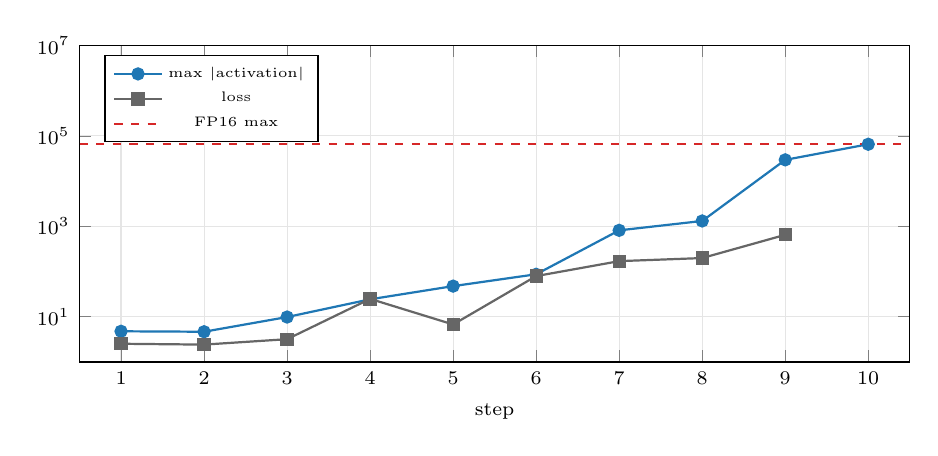
\begin{tikzpicture}
\begin{semilogyaxis}[width=\linewidth, height=5.6cm, xlabel={step}, xmin=0.5, xmax=10.5, ymin=1, ymax=1e7,
  xtick={1,...,10}, legend pos=north west, legend style={font=\tiny}, grid=major, grid style={black!10},
  tick label style={font=\scriptsize}, label style={font=\scriptsize}]
\addplot[validblue, thick, mark=*] coordinates {(1,4.766)(2,4.66)(3,9.852)(4,24.31)(5,47.59)(6,87)(7,815.5)(8,1315)(9,29570)(10,65440)};
\addlegendentry{max $|$activation$|$}
\addplot[black!60, thick, mark=square*] coordinates {(1,2.5254)(2,2.4189)(3,3.1881)(4,24.8335)(5,6.7435)(6,79.3333)(7,169.8536)(8,198.7644)(9,649.355)};
\addlegendentry{loss}
\addplot[nanred, dashed, thick, domain=0.5:10.5] {65504};
\addlegendentry{FP16 max}
\end{semilogyaxis}
\end{tikzpicture}
\end{column}
\end{columns}
\end{frame}

%-----------------------------------------------------------------------------
\begin{frame}[fragile]{The nixnan setup: three runs and a watcher}
\begin{lstlisting}[language=bash]
# pass 0: log all 50 kernel names (dummy whitelist: nothing instrumented) -> generate the lists
# pass 1: exceptions everywhere except 18 tile-based kernels
watch_nan.py logs/nixnan-exceptions.log -- env LD_PRELOAD=nixnan.so FUNCTION_BLACKLIST=blacklist.txt python train_fp16.py --lr 1
# pass 2: binade histogram + instruction, on the residual add and LayerNorm only
watch_nan.py logs/nixnan-climb.log -- env LD_PRELOAD=nixnan.so FUNCTION_WHITELIST=hist-whitelist.txt \
      BIN_SPEC_FILE=spec-climb.json HISTOGRAM=1 python train_fp16.py --lr 1
\end{lstlisting}
\begin{columns}[T]
\begin{column}{0.5\textwidth}
\textbf{\code{spec-climb.json}}
\begin{lstlisting}[language={}]
{ "count": 1, "doublings": 20,
  "f16 (record_inst)": [[9,9],...,[15,15]],
  "f32 (record_inst)": [[9,9],...,[15,15],[16,17]] }
\end{lstlisting}
\small one bin per binade $2^9$--$2^{15}$; report the first hit and the instruction
\end{column}
\begin{column}{0.48\textwidth}
\textbf{\code{watch_nan.py}}
\begin{itemize}\small
\item timestamps every line of output
\item first line matching \verb|#nixnan: error \[[^\]]*NaN|\\ $\to$ \code{WATCHER} line, \code{SIGKILL} the process group
\item subnormal and $\pm\infty$ reports don't stop it
\end{itemize}
\end{column}
\end{columns}
\end{frame}

%-----------------------------------------------------------------------------
\begin{frame}{Result: the timeline nixnan reports (\code{logs/SUMMARY.txt})}
\footnotesize
\begin{tabular}{rr>{\raggedright\arraybackslash}p{4.3cm}>{\raggedright\arraybackslash}p{3.0cm}>{\raggedright\arraybackslash}p{4.2cm}}
\toprule
step & loss & residual add (\code{CUDAFunctor_add<Half>}) & LayerNorm & exceptions \\
\midrule
1--6 & 2.5--79 & below $2^9$ & up to $2^{17}$ (FP32 $\sum(x-\mu)^2$) & none \\
7 & 169.9 & \textbf{$2^{9}$ ($\geq 512$)}, \code{FFMA} & $2^{17}$ & none \\
8 & 198.8 & \textbf{$2^{10}$ ($\geq 1{,}024$)} & $2^{17}$ & none \\
9 & 649.4 & \textbf{$2^{15}$ ($\geq 32{,}768$)}, 49k reports & $2^{17}$ & none \\
10 & --- & $2^{15}$, then \textcolor{infor}{$\pm\infty$} in \code{FFMA} & \textcolor{infor}{$-\infty$}, then \textcolor{nanred}{\textbf{\NaN}} & \textbf{run killed} \\
\bottomrule
\end{tabular}
\vspace{4mm}
\normalsize
\begin{itemize}
\item \textbf{Early warning}: the residual stream climbs binade by binade, 3 steps before overflow
\item Oracle maxima 815 / 1{,}315 / 29{,}570 fall in exactly these binades
\item FP16 bins never fire: PyTorch computes in \textbf{FP32} after loading FP16
\end{itemize}
\end{frame}

%-----------------------------------------------------------------------------
\stepframe{Steps 1--6: unstable, but finite}{}{}{loss $2.5 \to 3.2 \to 24.8 \to 6.7 \to 79.3$\\[1mm]
oracle: max $|$act$|$ $\leq 87$ (the logits, \code{head})\\[1mm]
\textbf{nixnan}
\begin{itemize}\scriptsize
\item no $\pm\infty$, no NaN
\item residual add: every operand $< 2^9$
\item LayerNorm FP32 bins climb to $2^{17}$: variance sums, FP32 only, harmless
\end{itemize}}

%-----------------------------------------------------------------------------
\stepframe{Step 7 (loss 169.9): the residual stream crosses 512}{n-proj/.style={st-warm}, n-add1/.style={st-warm, label={[tag, anchor=north east, yshift=-2.5mm, xshift=1.5mm]south west:{nixnan $\geq 2^{9}$}}}}{}{\textbf{nixnan} (histogram): the residual add's \code{FFMA ...c[0x0][0x164]...} hits the $2^9$ bin, 3{,}040 reports\\[1mm]
\textbf{oracle}: largest activation is \code{blocks.0.proj}'s output, 815\\[1mm]
\textcolor{black!60}{nixnan's bins don't say which of the 8 add calls; the oracle places it at block 0's first add}}

%-----------------------------------------------------------------------------
\stepframe{Step 8 (loss 198.8): $\geq 1{,}024$}{n-proj/.style={st-warm}, n-add1/.style={st-warm, label={[tag, anchor=north east, yshift=-2.5mm, xshift=1.5mm]south west:{nixnan $\geq 2^{10}$}}}}{}{\textbf{nixnan}: the add's $2^{10}$ bin fires (1{,}292 reports)\\[1mm]
\textbf{oracle}: \code{blocks.0.proj} output 1{,}315\\[1mm]
weights keep growing: max $|w|$ 6.5 $\to$ 23.7}

%-----------------------------------------------------------------------------
\stepframe{Step 9 (loss 649.4): $\geq 32{,}768$, one binade from overflow}{n-proj/.style={st-hot}, n-add1/.style={st-hot, label={[tag, anchor=north east, yshift=-2.5mm, xshift=1.5mm]south west:{nixnan $\geq 2^{15}$}}}}{}{\textbf{nixnan}: the add's $2^{15}$ bin fires, 49{,}144 reports\\[1mm]
\textbf{oracle}: \code{blocks.0.proj} output 29{,}570\\[1mm]
FP16 max is 65{,}504: the next doubling overflows.\\[1mm]
\textbf{Still no exception report}: only the histogram sees this coming}

%-----------------------------------------------------------------------------
\stepframe{Step 10, \textcircled{\scriptsize 1}: the proj GEMM overflows}{n-proj/.style={st-inf, dashed, label={[tag]north:{FP32 acc.\ $> 65{,}504 \to \pm\infty$}}}, e-proj/.style={e-inf}}{}{\code{blocks.0.proj}: FP16 GEMM, FP32 accumulate\\[1mm]
7{,}870 outputs exceed 65{,}504 and round to $\pm\infty$ on the FP16 store (the largest finite one: 65{,}440)\\[1mm]
\textbf{nixnan: silent here}. GEMMs are blacklisted (padding-lane false positives), so it sees the $\infty$ one kernel later}

%-----------------------------------------------------------------------------
\stepframe{Step 10, \textcircled{\scriptsize 2}: the residual add reads $\pm\infty$}{n-proj/.style={st-inf, dashed}, e-proj/.style={e-inf}, n-add1/.style={st-inf, label={[tag, anchor=north east, yshift=-2.5mm, xshift=1.5mm]south west:{\code{FFMA} op 1 $=\pm\infty$}}}, e-a1/.style={e-inf}, e-skip2/.style={e-inf}}{}{\textbf{nixnan}:\\
\code{[infinity] operand 1 of}\\ \code{FFMA R9, R9, c[0x0][0x164], R8}\\
\code{[infinity] operand 0 ...}\\[1mm]
$d = \alpha\, b + a$: op 1 $= b$ = proj output, op 0 = the sum. Six reports, three \code{FFMA}s, $+\infty$ and $-\infty$\\[1mm]
the add \emph{reads} the $\infty$; it doesn't create it}

%-----------------------------------------------------------------------------
\stepframe{Step 10, \textcircled{\scriptsize 3}: LayerNorm makes the first NaN, and the run is killed}{n-proj/.style={st-inf, dashed}, e-proj/.style={e-inf}, n-add1/.style={st-inf}, e-a1/.style={e-inf}, n-ln2/.style={st-nan, label={[tag, anchor=south east]north west:{$(-\infty)-(-\infty)$}}}, n-fc1/.style={st-off}, n-gelu/.style={st-off}, n-fc2/.style={st-off}, n-add2/.style={st-off}, n-blk13/.style={st-off}, n-lnf/.style={st-off}, n-head/.style={st-off}, n-ce/.style={st-off}, n-loss/.style={st-off}, e-mlp/.style={e-off}, e-out/.style={e-off}, e-skip2/.style={e-off}}{}{\textbf{nixnan}, in \code{ln2}:\\
\code{[-infinity] FADD R18, R19, -R16}\\
\code{[-infinity] FFMA R16, R18, R15, R16}\\
\quad$\to$ row mean $\mu = -\infty$\\
\code{[NaN] operand 0 of}\\ \code{FADD R0, R19, -R16}\\
\quad$x-\mu = (-\infty)-(-\infty)$\\[1mm]
\textbf{\code{WATCHER}: SIGKILL}, 54.0 s into the run. Nothing after \code{ln2} runs}

%-----------------------------------------------------------------------------
\stepframe{Without the watcher: NaN everywhere}{n-proj/.style={st-inf}, e-proj/.style={e-inf}, n-add1/.style={st-inf}, e-a1/.style={e-inf}, n-ln2/.style={st-nan}, n-fc1/.style={st-nan}, n-gelu/.style={st-nan}, n-fc2/.style={st-nan}, n-add2/.style={st-nan}, n-blk13/.style={st-nan}, n-lnf/.style={st-nan}, n-head/.style={st-nan}, n-ce/.style={st-nan}, n-loss/.style={st-nan}, e-mlp/.style={e-nan}, e-out/.style={e-nan}, e-skip2/.style={e-inf}}{}{(oracle run, no nixnan)\\[1mm]
the NaN rows of \code{ln2} go through the MLP; $\infty + \mathrm{NaN}$ in the second add; attention mixes the NaN rows into later positions\\[1mm]
\textbf{loss $=$ NaN} at step 10, gradients NaN\\[1mm]
\code{train_fp16.py} stops at the non-finite loss}

%-----------------------------------------------------------------------------
\begin{frame}[fragile]{Step 10, report by report}
\begin{lstlisting}[language={}]
[54.0s] error [infinity]  operand 1 of FFMA R9, R9, c[0x0][0x164], R8   ; add kernel
[54.0s] error [infinity]  operand 0 of FFMA R9, R9, c[0x0][0x164], R8   ; (3 FFMAs, +inf and -inf)
[54.0s] error [-infinity] operand 1 of FADD R18, R19, -R16              ; LayerNorm
[54.0s] error [-infinity] operand 0 of FFMA R16, R18, R15, R16
[54.0s] error [-infinity] operand 1 of FADD R0, R19, -R16
[54.0s] error [-infinity] operand 2 of FADD R0, R19, -R16
[54.0s] error [NaN]       operand 0 of FADD R0, R19, -R16
[54.0s] WATCHER: first nixnan NaN report -- killing the run
\end{lstlisting}
\begin{itemize}\small
\item Operand 0 $=$ destination, 1, 2, \ldots{} $=$ sources
\item Add: $d=\alpha\cdot b + a$ with $\alpha=$ \code{c[0x0][0x164]}; $b$ = \code{proj} output $=\infty$. \textbf{The add reads the $\infty$; it doesn't create it}
\item LayerNorm: running mean $\mu\to-\infty$, then $x-\mu = (-\infty)-(-\infty) = \textbf{\NaN}$
\end{itemize}
\end{frame}

%-----------------------------------------------------------------------------
\begin{frame}[fragile]{Obstacle 1: false NaNs in a healthy step 1}
Instrument everything $\Rightarrow$ the watcher fires at \textbf{step 1}, while every tensor is finite and $\leq 5$.
\vspace{1mm}
\begin{lstlisting}[language={}]
error [NaN,subnormal] operand 1 of HMMA.16816.F32 R20, R48.reuse, R46, R20 ; void cutlass::Kernel2  (f16)
\end{lstlisting}
GEMMs blacklisted $\Rightarrow$ next stop, \code{softmax_warp_forward} in \code{cross_entropy}:
\begin{lstlisting}[language={}]
error [-infinity] operand 0 of FFMA R8, R7, 1.4426950216293334961, -R8 ; void   (log2 e)
error [NaN]       operand 0 of FADD R7, -R12, R7 ; void
\end{lstlisting}
\begin{itemize}\small
\item \textbf{Padding lanes}: tile lanes outside the tensor compute on stale bits (GEMM) or on $-\infty$ padding (softmax: $-\infty-(-\infty)$), and are never stored
\item Same effect as flash attention (\code{PyTorch_Instrumentation/PyT.md})
\item Fix: blacklist 18 tile kernels (cuBLAS, CUTLASS, splitK, flash, warp softmax).\\
  A GEMM overflow is still caught, by the next kernel
\end{itemize}
\end{frame}

%-----------------------------------------------------------------------------
\begin{frame}[fragile]{Obstacles 2--4: what the run says about nixnan}
\begin{columns}[T]
\begin{column}{0.5\textwidth}
\textbf{2. \code{MAX_ERRORS} can't stop at a NaN}
\begin{itemize}\scriptsize
\item counts every report, subnormals included
\item FP16 GEMMs report subnormals at step 1; GELU at step 8
\item $\to$ \code{watch_nan.py}; suggestion: \code{MAX_NANS} / category mask
\end{itemize}
\vspace{2mm}
\textbf{4. Truncated kernel names}
\begin{itemize}\scriptsize
\item \code{cut_kernel_name}: \code{find_first_of("<(")}
\item LayerNorm prints as \code{void at::native::}, softmax as \code{void }
\item identifiable only because pass 2 instruments 2 kernels
\end{itemize}
\end{column}
\begin{column}{0.48\textwidth}
\textbf{3. \code{HISTOGRAM=1} on all kernels segfaults}
\begin{lstlisting}[language=C++]
// src/recording.cu:88  recorder::mk_entry
inst_info[current_entry].instr = instr;
...
return current_entry++;   // no bound check
// src/nixnan.cu:71
#define TABLE_SIZE (1l << 17)
\end{lstlisting}
\begin{itemize}\scriptsize
\item gdb: \code{SIGSEGV} in \code{mk_entry}, \code{FFMA} of \code{cutlass::Kernel2}
\item large GEMMs overflow the $2^{17}$-entry table
\item $\to$ histogram whitelist of 2 kernels; nixnan left unmodified
\end{itemize}
\end{column}
\end{columns}
\end{frame}

%-----------------------------------------------------------------------------
\begin{frame}{Reproducibility and caveats}
\begin{itemize}
\item \code{./run_nixnan.sh}: $\approx$5 min on an RTX 3090; full rerun gave
  \begin{itemize}
  \item the same losses, the same histogram timeline, the same step-10 \code{FFMA}/\code{FADD} sequence
  \item only difference: \emph{which} LayerNorm instruction prints the first \NaN{}\\
    (\code{FADD R0,R19,-R16} or the \code{FFMA R17,R18,R0,R17} that consumes it), warp order
  \end{itemize}
\item LayerNorm's FP32 bins reach $2^{17}$ from step 6 on: variance sums, harmless.\\
  \textbf{The residual add is the signal to watch}
\item nixnan cannot see \emph{inside} the blacklisted GEMM; the oracle names it
\item Environment: PyTorch 2.6.0+cu124, CUDA 12.4, sm\_86, NVBit 1.8, nixnan unmodified
\end{itemize}
\end{frame}

%-----------------------------------------------------------------------------
\begin{frame}{Takeaways}
\begin{itemize}
\item Without touching the program, nixnan gave:
  \begin{itemize}
  \item the \textbf{climb}: residual stream $\geq 512$, $\geq 1{,}024$, $\geq 32{,}768$ in steps 7, 8, 9
  \item the \textbf{first $\infty$}: the residual add's \code{FFMA}, operand 1 (an overflowed GEMM output)
  \item the \textbf{first \NaN}: LayerNorm's $x-\mu = (-\infty)-(-\infty)$, then the run was killed
  \end{itemize}
\item Aiming it took a model of the program: which kernels are tile-based, which carry the
  residual stream, and that FP16 is computed as FP32
\item Tool improvements suggested by this run: padding-lane awareness, \code{MAX_NANS},
  a bounded instruction table, full kernel names
\item Standard fixes break one link each: lower lr / AdamW, clipping, master weights +
  \code{GradScaler}, or BF16
\end{itemize}
\vspace{2mm}
\scriptsize Report: \code{fp16-divergence/latex/report.pdf}\quad Code and logs: \code{flash-attn-expt/fp16-divergence/}
\end{frame}

%-----------------------------------------------------------------------------
\begin{frame}{Closing (1/2): nixnan's exception reports, on the blocks}
\begin{columns}[c]
\begin{column}{0.60\textwidth}\centering\resizebox{\linewidth}{!}{\gptarch[n-emb/.style={st-blind}, n-qkv/.style={st-blind}, n-proj/.style={st-blind}, n-fc1/.style={st-blind}, n-fc2/.style={st-blind}, n-head/.style={st-blind}, n-flash/.style={st-blind}, n-ce/.style={st-blind}, n-proj/.style={st-blind, st-inf, dashed}, n-add1/.style={st-inf}, n-ln2/.style={st-nan}]{%
  \badge{qkv}{1}\badge{proj}{1}\badge{fc1}{1}\badge{fc2}{1}\badge{head}{1}\badge{emb}{1}
  \badge{flash}{2}\badge{ce}{3}\badge{gelu}{4}\badge{add1}{5}\badge{ln2}{6}}}
\end{column}
\begin{column}{0.39\textwidth}\scriptsize
\begin{enumerate}\setlength{\itemsep}{1pt}
\item GEMMs, step 1: \code{[NaN]} in \code{HMMA} op 1, padding lanes $\to$ blacklisted
\item flash: padding-lane NaNs $\to$ blacklisted
\item warp softmax, step 1: $-\infty-(-\infty)$ on padding $\to$ blacklisted
\item GELU backward, steps 8--9: 18 subnormals, harmless
\item step 10: \code{[infinity]} op 1, op 0 of\\ \code{FFMA R9,R9,c[0x0][0x164],R8}
\item step 10: \code{[-infinity]} in the mean update, then\\ \code{[NaN]} op 0 of \code{FADD R0,R19,-R16}\\ $\to$ \textbf{\code{WATCHER} kill}
\end{enumerate}
\end{column}
\end{columns}
\end{frame}

%-----------------------------------------------------------------------------
\begin{frame}{Closing (2/2): nixnan's histogram, on the blocks}
\begin{columns}[c]
\begin{column}{0.60\textwidth}\centering\resizebox{\linewidth}{!}{\gptarch[n-emb/.style={st-blind}, n-qkv/.style={st-blind}, n-flash/.style={st-blind}, n-proj/.style={st-blind}, n-fc1/.style={st-blind}, n-gelu/.style={st-blind}, n-fc2/.style={st-blind}, n-head/.style={st-blind}, n-ce/.style={st-blind}, n-add1/.style={st-watch}, n-add2/.style={st-watch}, n-ln1/.style={st-watch}, n-ln2/.style={st-watch}, n-lnf/.style={st-watch}]{%
  \badge{add1}{1}\badge{add2}{1}\badge{ln1}{2}\badge{ln2}{2}\badge{lnf}{2}\badge[south east]{add1}{3}\badge[south east]{ln2}{4}}}
\end{column}
\begin{column}{0.39\textwidth}\scriptsize
Blue: the 2 whitelisted kernels (all instances). Gray: not instrumented.
\begin{enumerate}\setlength{\itemsep}{1pt}
\item add, FP32, \code{FFMA ...c[0x0][0x164]...}:\\ $2^{9}$ (step 7), $2^{10}$ (8), $2^{15}$ (9)\\ \textbf{the early warning}
\item LayerNorm, FP32: $2^{10}$ (4), $2^{13}$ (5), $2^{17}$ (6--9): variance sums, harmless
\item step 10: $\pm\infty$ in the add
\item step 10: $-\infty$, then NaN, in \code{ln2} $\to$ kill
\end{enumerate}
FP16 bins never fire: both kernels compute in FP32.
\end{column}
\end{columns}
\end{frame}

\end{document}
